\documentclass{article}

% Language setting
\usepackage[english]{babel}

% Set page size and margins
% Replace `letterpaper' with `a4paper' for UK/EU standard size
\usepackage[letterpaper,top=2cm,bottom=2cm,left=3cm,right=3cm,marginparwidth=1.75cm]{geometry}

% Useful packages
\usepackage{amsmath}
% --- Code listings ---
\usepackage{listings}
\usepackage{xcolor}
\definecolor{codegreen}{rgb}{0,0.6,0}
\definecolor{codegray}{rgb}{0.5,0.5,0.5}
\definecolor{codepurple}{rgb}{0.58,0,0.82}
\definecolor{backcolour}{rgb}{0.95,0.95,0.92}

\lstdefinestyle{mystyle}{
    backgroundcolor=\color{backcolour},   
    commentstyle=\color{codegreen},
    keywordstyle=\color{magenta},
    numberstyle=\tiny\color{codegray},
    stringstyle=\color{codepurple},
    basicstyle=\ttfamily\footnotesize,
    breakatwhitespace=false,         
    breaklines=true,                 
    captionpos=b,                    
    keepspaces=true,                 
    numbers=left,                    
    numbersep=5pt,                  
    showspaces=false,                
    showstringspaces=false,
    showtabs=false,                  
    tabsize=2
}

\lstset{style=mystyle}
% --- End Code Listings
\usepackage{graphicx}
\usepackage{float}
\usepackage{caption}
\captionsetup{labelformat=empty} 
% \usepackage{subcaption}
\usepackage[colorlinks=true, allcolors=blue]{hyperref}
\graphicspath{{./figures/}}

\title{ECE 637 Lab - Image Restoration}
\author{Colin Braun}

\begin{document}
\maketitle

\section{Minimum Mean Square Error (MMSE) Linear Filters}
\begin{figure}[H]
    \centering
    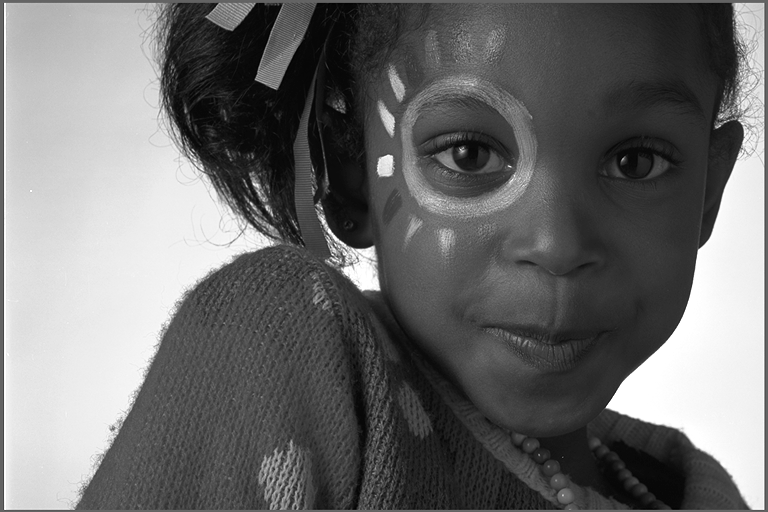
\includegraphics[width=1\textwidth]{../img14g.png}
    \caption{Original img14g.tif.}
\end{figure}
\begin{figure}[H]
    \centering
    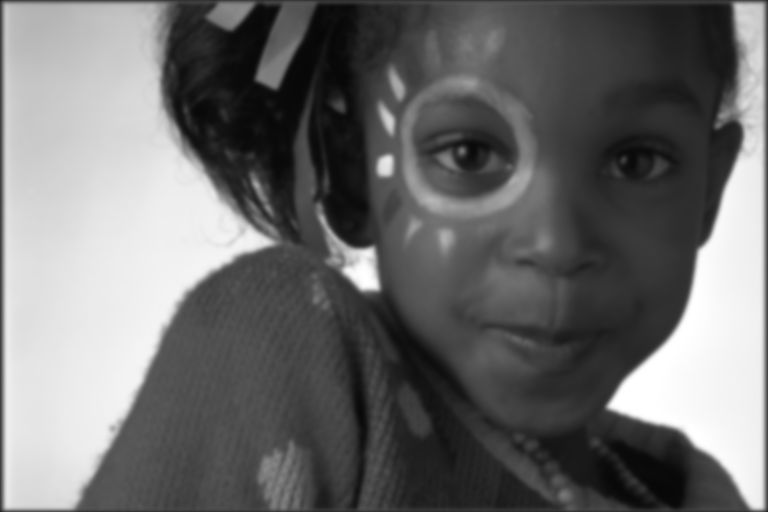
\includegraphics[width=1\textwidth]{../img14bl.png}
    \caption{Original img14bl.tif.}
\end{figure}
\begin{figure}[H]
    \centering
    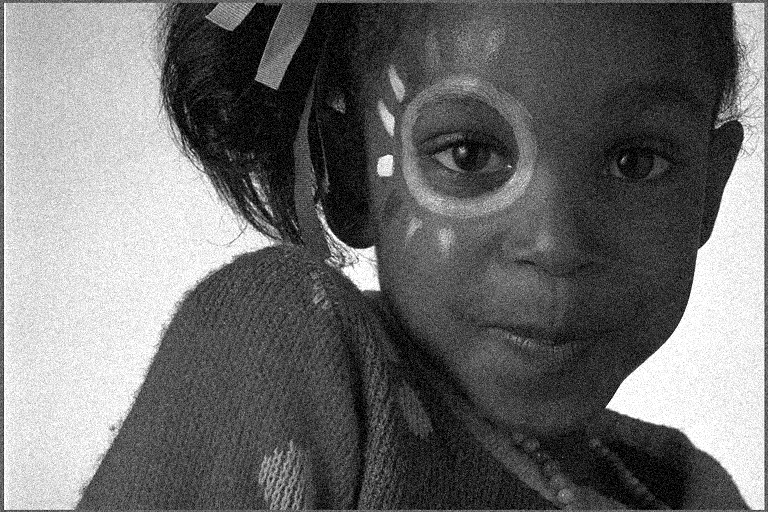
\includegraphics[width=1\textwidth]{../img14gn.png}
    \caption{Original img14gn.tif.}
\end{figure}
\begin{figure}[H]
    \centering
    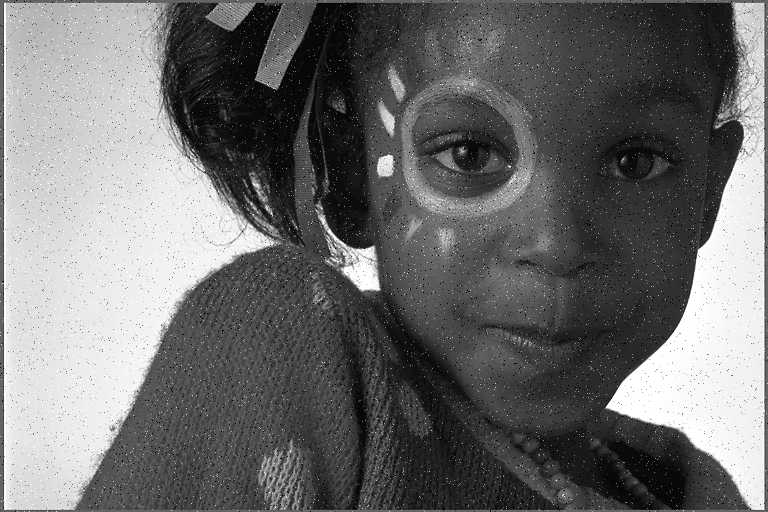
\includegraphics[width=1\textwidth]{../img14sp.png}
    \caption{Original img14sp.tif.}
\end{figure}
\begin{figure}[H]
    \centering
    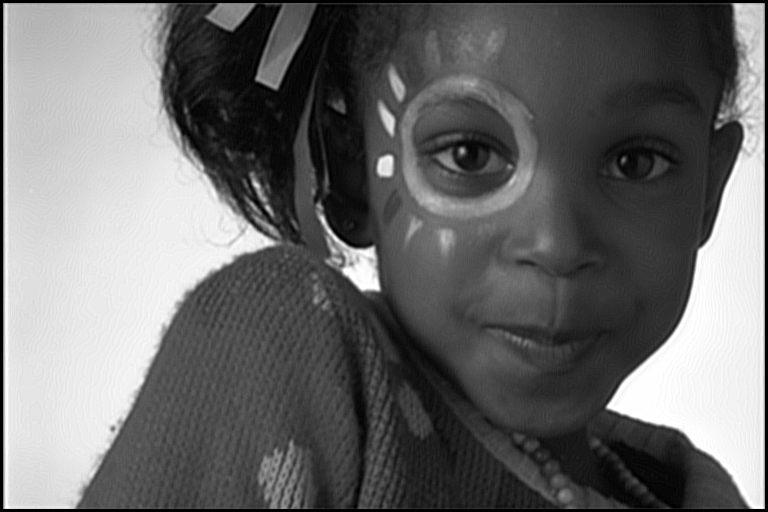
\includegraphics[width=1\textwidth]{../1-img14bl-restored.png}
    \caption{Restored img14bl.tif.}
\end{figure}
\begin{figure}[H]
    \begin{equation*}
        \begin{bmatrix}
        1.5208 & -1.6833 & -0.0147 & 0.9993 & -0.2206 & 0.0671 & 0.5672\\
        -0.2197 & -1.3117 & -0.3552 & -0.4407 & -1.1395 & -0.4067 & -0.4302\\
        1.3415 & -0.97 & 0.7195 & 2.3861 & 0.6888 & -1.1164 & 0.4174\\
        -1.1754 & -0.0361 & 1.2484 & 1.8966 & 0.5231 & -0.6413 & -0.3591\\
        0.3286 & -0.8734 & 0.1385 & 0.9866 & 0.4403 & -1.1208 & 0.733\\
        -0.578 & -0.7402 & 0.5593 & 0.1056 & -0.636 & -2.1178 & 1.3349\\
        1.0864 & -0.8139 & 0.2833 & -0.9683 & 1.0474 & -0.0205 & -0.0308\\
        \end{bmatrix}
    \end{equation*}
\caption{MMSE filter for img14bl.tif.}
\end{figure}
\begin{figure}[H]
    \centering
    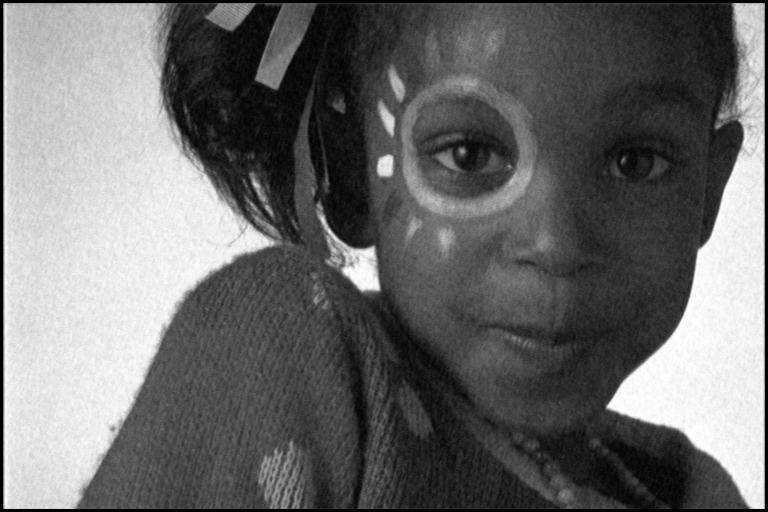
\includegraphics[width=1\textwidth]{../1-img14gn-restored.png}
    \caption{Restored img14gn.tif.}
\end{figure}
\begin{figure}[H]
    \begin{equation*}
        \begin{bmatrix}
        -0.0106 & -0.0088 & -0.0079 & 0.0365 & 0.0359 & 0.0115 & 0.0035\\
        0.0354 & 0.0035 & 0.0111 & 0.0405 & 0.0461 & -0.0169 & -0.0016\\
        -0.0184 & 0.0214 & 0.0657 & 0.0963 & 0.0337 & -0.0189 & -0.0201\\
        -0.0106 & 0.0043 & 0.1015 & 0.1991 & 0.0717 & 0.0155 & -0.0015\\
        -0.0004 & 0.0407 & 0.0371 & 0.0851 & 0.0333 & 0.007 & 0.0119\\
        -0.0285 & 0.0128 & 0.0258 & 0.0179 & 0.0019 & 0.025 & -0.0105\\
        -0.0284 & 0.0007 & 0.0164 & 0.012 & 0.0117 & 0.0066 & 0.0102\\
        \end{bmatrix}
    \end{equation*}
\caption{MMSE filter for img14gn.tif.}
\end{figure}
\begin{figure}[H]
    \centering
    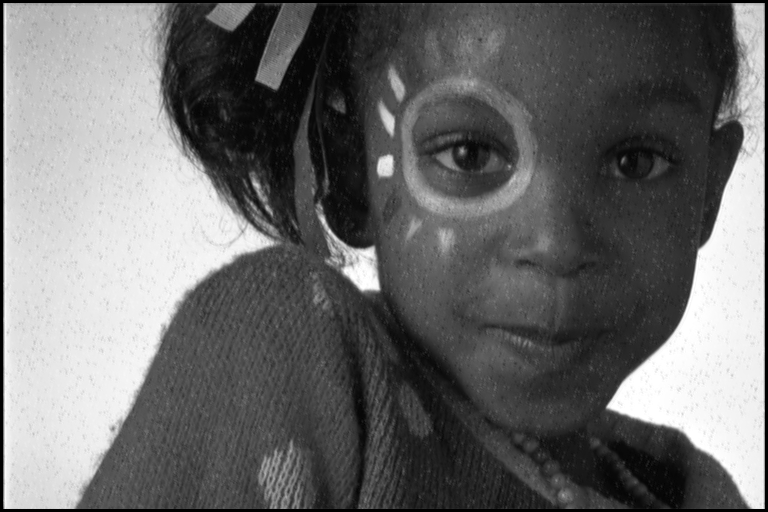
\includegraphics[width=1\textwidth]{../1-img14sp-restored.png}
    \caption{Restored img14sp.tif.}
\end{figure}
\begin{figure}[H]
    \begin{equation*}
        \begin{bmatrix}
        0.026 & -0.035 & 0.025 & 0.043 & 0.046 & 0.005 & -0.\\
        0.023 & 0.005 & -0.003 & 0.024 & 0.037 & -0.014 & -0.002\\
        -0.001 & -0.017 & 0.069 & 0.129 & 0.006 & -0.017 & -0.008\\
        0.018 & -0.012 & 0.079 & 0.183 & 0.086 & -0.006 & 0.007\\
        -0.011 & 0.029 & 0.057 & 0.111 & 0.061 & -0.011 & 0.014\\
        -0.023 & 0.013 & 0.018 & 0.023 & 0.028 & 0.001 & -0.02\\
        -0.037 & 0.016 & 0.018 & -0.012 & -0.002 & 0.017 & 0.016\\
        \end{bmatrix}
    \end{equation*}
\caption{MMSE filter for img14sp.tif.}
\end{figure}

\section{Weighted Median Filtering}
\begin{figure}[H]
    \centering
    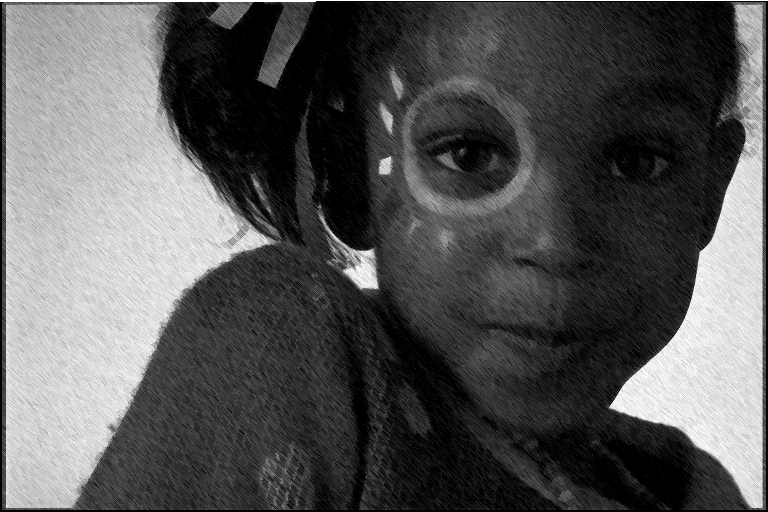
\includegraphics[width=1\textwidth]{../2-img14gn-corrected.png}
    \caption{Median filter applied to img14gn.tif.}
\end{figure}
\begin{figure}[H]
    \centering
    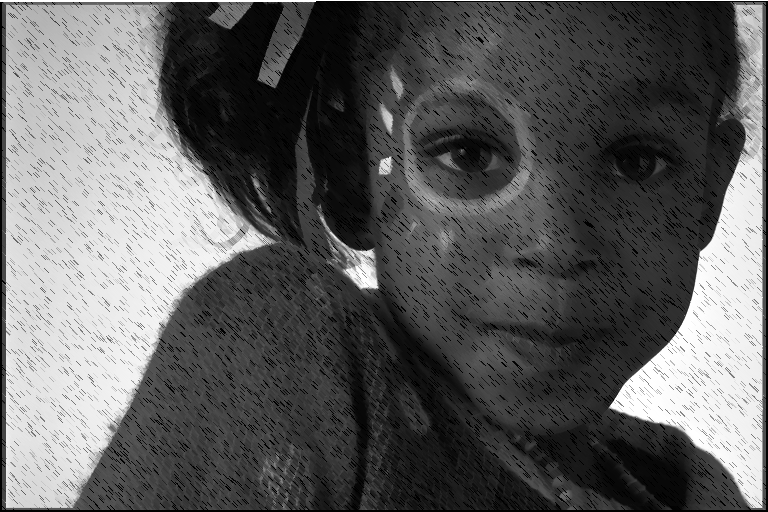
\includegraphics[width=1\textwidth]{../2-img14sp-corrected.png}
    \caption{Median filter applied to img14sp.tif.}
\end{figure}

\large{C Code (section2.c, util.c)}

section2.c:
\lstinputlisting[language=C]{../section2.c}

util.c:
\lstinputlisting[language=C]{../util.c}

\end{document}
